\section{Processi primari}
\subsection{Acquisizione}
\textit{Zucchetti S.p.A.} richiede la realizzazione di un progetto creativo riguardante lo sviluppo di un sistema Captcha attraverso l'esposizione della lettera di presentazione \textit{"CAPTCHA: Umano o Sovrumano?"} in data 18 ottobre 2022.

\subsection{Fornitura}
Successivamente alla presentazione dei capitolati \textit{CatchEmAll} si riunisce per valutare le proposte e le opinioni dei componenti del team: attraverso un processo di valutazione (inizialmente generico poi specifico, riassunto nella sezione \textit{Motivazione scelta capitolato} del documento \href{https://github.com/catchEmAll-SWE/catchEmAll-Docs/blob/main/Assegnazione appalti/LetteraCandidatura.pdf}{lettera di presentazione}) emerge una preferenza per il progetto proposto dal referente Dr. Gregorio Piccoli.  
\newline
In seguito viene schedulata una riunione con il proponente con l'obiettivo di approfondire e consolidare le richieste. 
\newline
In data 28 ottobre 2022 viene inviata al committente la \textit{lettera di presentazione} il quale, in seguito ad una richiesta di modifica delle tempistiche di consegna, ci aggiudica l'appalto.

\subsection{Sviluppo}
    \subsubsection{Versionamento}
    GitHub è lo strumento utilizzato dal gruppo per il versionamento del codice.
    \newline Il team è identificato in tale piattaforma come organizzazione (\href{https://github.com/catchEmAll-SWE}{vedi}).
    Inoltre, al fine di documentare il più possibile, ogni commit che porta valore al progetto contiene il riferimento al ticket che completa (totalmente o anche solo parzialmente). 
    
    \subsubsection{GitHub Workflow}
    Tutti i titoli e le descrizioni dei commit devono essere fatti in inglese per conformità tra essi.
    \newline Il Workflow viene gestito concorrentemente da GitHub e JIRA, in JIRA vengono create ed organizzate le issue, una volta fatto ciò si procede attraverso github alla creazione del branch relativo alla issue da risolvere.\\
    Tale ramo ha nome codificato come:
    \begin{lstlisting}
    CEA-num-titolo-della-issue
    \end{lstlisting}
    Questo permette di identificare titolo e numero della issue di appartenenza. Una volta fatto ciò viene creato un \textbf{primo commit}, nel cui messaggio è specificata l'avvenuta presa in carico della issue, la quale dovrà passare dallo stato "to do" allo stato "in progress"\\
    Ciò è garantito dal suddetto commit message contenente la stringa:
    \begin{lstlisting}
    CEA-num #open <testo aggiuntivo>
    \end{lstlisting}
    Una volta fatto ciò è possibile lavorare liberamente sul proprio ramo di feature.
    \newline \textbf{Ad ogni} aggiornamento dell'attività svolta si dovrà fare riferimento alla issue e specificare il tempo impiegato per lo svolgimento di tale attività includendo nella descrizione:
    \begin{itemize}
        \item Visual Studio Code:
        \begin{figure}[h!]
            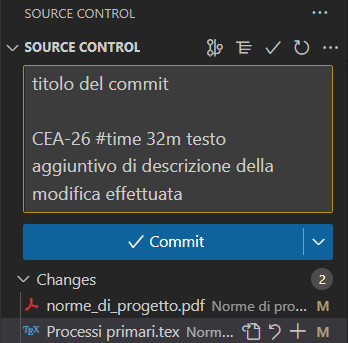
\includegraphics[scale=0.65]{img/visual_code_example.png}
        \end{figure}
        \item Git Bash:
        \begin{lstlisting}
        git commit -m "titolo del commit" -m "CEA-26 #time 32m ..."
        \end{lstlisting}
    \end{itemize}
    Comando generico da aggiungere nel corpo del messaggio, non nel titolo:
    \begin{lstlisting}
    CEA-num #time ww dd hh mm <testo aggiuntivo>
    \end{lstlisting}
    Così facendo è permesso specificare a scelta settimane, giorni, ore e minuti di lavoro, ad esempio:
    \begin{lstlisting}
    CEA-26 #time 1h aggiunto github Workflow
    \end{lstlisting}
    Ciò aggiunge 1h alle ore di lavoro impiegate per la issue con ID CEA-26, e come testo aggiuntivo per il commit "aggiunto github Workflow", ignorato da JIRA.\\
    Una volta terminata l'attività, sarà necessario passare allo stato di revisione, il quale permette di verificare il corretto svolgimento del compito eseguito. Questo è permesso da un ultimo commit prima della revisione, con messaggio da includere nella descrizione(non titolo):
    \begin{lstlisting}
    CEA-num #review #time ww dd hh mm <testo aggiuntivo>
    \end{lstlisting}
    Questo permette lo spostamento della issue dallo stato "in progress" allo stato "in review".\\
    Per permettere la revisione è necessario aprire una pull request, il titolo deve corrispondere al nome del branch.
    Una volta revisionata la issue, se presenta qualche problema può essere spostata allo stato "in progress" dal pannello JIRA. Altrimenti attraverso pull request nel ramo "main" e con comando posto \textbf{nel TITOLO del commit di chiusura della pull request}:
    \begin{lstlisting}
    CEA-num #close <testo aggiuntivo>
    \end{lstlisting}
    Viene chiusa. Una volta chiusa sempre dalla pul request su github, \textbf{si elimina il ramo di feature} creato precedentemente.
    \begin{figure}[h!]
        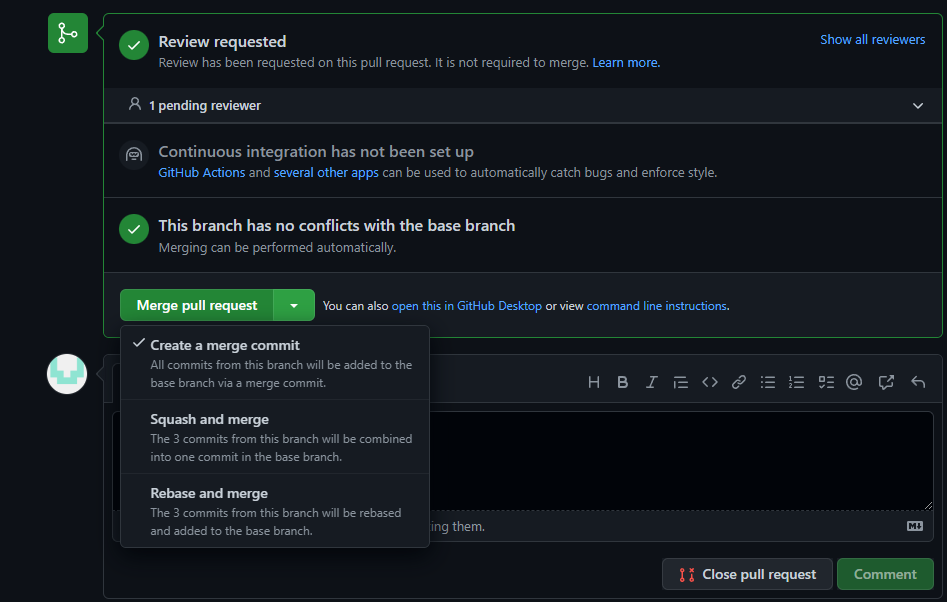
\includegraphics[width=15cm]{img/git_pull_request.png}
        \newline 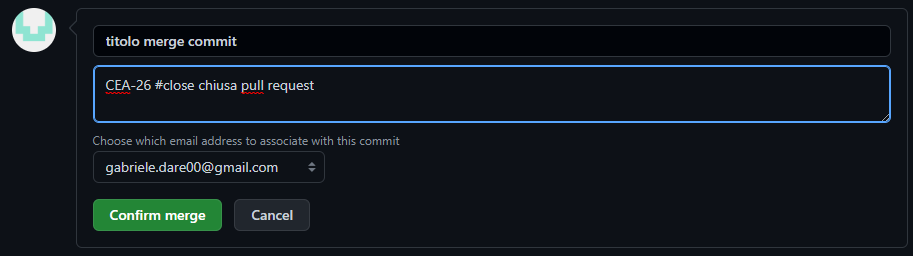
\includegraphics[width=15cm]{img/git_pull_request_commit.png}
    \end{figure}
    \clearpage

    \subsubsection{Issues tracking}
    JIRA, piattaforma che offre un servizio di \textit{Issue Tracking} è il supporto scelto vista la qualità ed il numero dei servizi e delle estensioni che offre.
    \newline
    La definizione dei ticket è regolata dalla seguente convenzione:
    \begin{itemize}
        \item titolo e descrizione devono, oltre ad essere sempre presenti, eplicitare in maniera chiara il problema
        \item utilizzo di label
        \item stima del lavoro necessario al completamento
        \item corretto utilizzo di ereditarietà (rapporti di parentela)
    \end{itemize}
    Si è deciso di di adottare il framework \textbf{Scrum} per la gestione del ciclo di sviluppo del progetto con le seguenti caratteristiche:
    \begin{itemize}
        \item sprint della durata di una settimana
        \item utilizzo di una board avente 4 stati:
            \begin{itemize}
                \item to do
                \item in progress
                \item in review (ogni ticket deve essere validato da uno o più componenti del gruppo per essere considerato chiuso)
                \item done
            \end{itemize}
    \end{itemize}

    JIRA dispone di un'integrazione con github che fornisce un meccanismo chiamato \textit{smart commit} il quale permette la transizione dei ticket da uno stato ad un'altro attraverso comandi posti nei commit stessi, la sintassi utilizzata è la seguente
    \begin{lstlisting}
    CEA-number #command <message body describing the commit>
    \end{lstlisting}
    Tra i comandi troviamo:
    \begin{itemize}
        \item \textbf{open}: permette di spostarsi da una issue nello stadio "to do" oppure "in review" allo stadio "in progress"
        \item \textbf{review}: permette lo spostamento della issue dallo stadio "in progress" oppure "done" allo stadio "in review"
        \item \textbf{close}: premette di spostarsi dallo stadio "in review" allo stadio "done"
        \item \textbf{close-no-rev}: permette in casi eccezionali di passare direttamente dallo stadio "in progress" allo stadio "done"
    \end{itemize}
    
